\section{Obiettivi di Qualità}
Il gruppo \gruppo\ ha ritenuto importante fissare alcuni obbiettivi di qualità da perseguire nel prodotto finale e nei processi di realizzazione, questo per garantire una migliore e più efficace soddisfazione dei requisiti richiesti nel capitolato d'appalto.
\subsection{Qualità dei Processi}

Per garantire la qualità del prodotto è necessario perseguire la qualità dei processi che lo definiscono. Per fare questo il team \gruppo\ ha deciso di adottare lo standard ISO/IEC$_G$ 15504 denominato SPICE$_G$ (Software Process Improvement Capability Determination), il quale definisce il modello denominato SPY$_G$ (SW Process Assessment \& Improvement, vedi Figura 1), per la valutazione dei processi in un'organizzazione del settore IT (Information Technology).\\
\begin{figure}[h!]
		\centering
		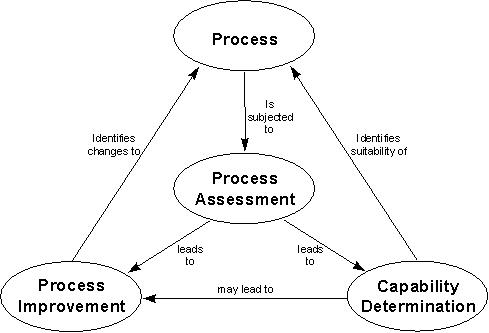
\includegraphics[scale=.6]{img/Spy.png}
		\caption{Modello SPY}
		\label{fig:ModelloSpy}
\end{figure}
\\Lo standard identifica e definisce nove attributi di qualità:
\smallskip
\begin{enumerate}
    \item \textbf{Process performance attribute}: un processo raggiunge i suoi obiettivi, trasformando input identificabili in output identificabili;
    \item \textbf{Performance management attribute}: l'attuazione di un processo è pianificata e controllata al fine di produrre risultati che rispondano agli obiettivi attesi;
    \item \textbf{Work product management attribute}: capacità del processo di elaborare un prodotto documentato, controllato e verificato;
    \item \textbf{Process definition attribute}: l'esecuzione del processo si basa su standard di processo per raggiungere i propri obiettivi;
    \item \textbf{Process resource attribute}: capacità del processo di attingere a risorse tecniche e umane appropriate per essere attuato efficacemente;
    \item \textbf{Process measurement attribute}: i risultati raggiunti e le misure rilevate durante l'attuazione di un processo sono stati usati per assicurarsi che l'attuazione di tale processo supporti efficacemente il raggiungimento di specifici obiettivi;
    \item \textbf{Process control attribute}: il processo viene controllato attraverso la raccolta, analisi ed utilizzo delle misure di prodotto e di processo, al fine di correggere, se necessario, le sue modalità di attuazione;
    \item \textbf{Process change attribute}: i cambiamenti strutturali, di gestione e di esecuzione vengono gestiti in modo controllato;
    \item \textbf{Continuous improvement attribute}: le modifiche al processo sono identificate e implementate per garantire il miglioramento continuo nella realizzazione degli obiettivi di business dell'organizzazione.
\end{enumerate}
\smallskip
La norma definisce poi quattro livelli di possesso di ciascun attributo:
\smallskip
\begin{itemize}
	\item \textbf{N} - Non posseduto (0\%-15\% di possesso): non c'è evidenza oppure ce n'è poca del possesso di un attributo;
	\item \textbf{P} - Parzialmente posseduto (16\%-50\% di possesso): vi è evidenza di approccio sistematico al raggiungimento del possesso di un attributo, ma alcuni aspetti del possesso possono essere non prevedibili;
    \item \textbf{L} - Largamente posseduto (51\%-85\% di possesso): vi è evidenza di approccio sistematico al raggiungimento di un significativo livello di possesso di un attributo, ma l'attuazione del processo può variare nelle diverse unità operative della organizzazione;
	\item \textbf{F} - (Fully) Pienamente posseduto (86\%-100\% di possesso): vi è evidenza di un approccio completo e sistematico e di un pieno raggiungimento del possesso dell'attributo, non esistono significative differenze nel modo di attuare il processo tra le diverse unità operative.
\end{itemize}
\smallskip
Vi sono infine cinque livelli di maturità di processi:
\smallskip
\begin{itemize}
	\item \textbf{Livello 0 - Processo incompleto}: il processo non è implementato o non raggiunge gli obiettivi. Non vi è evidenza di approcci sistematici agli
	attributi definiti;
	\item \textbf{Livello 1 - Processo semplicemente attuato}: il processo viene messo in atto e raggiunge i suoi obiettivi. Non vi è evidenza di un approccio sistematico ad alcuno degli attributi definiti. Il raggiungimento di questo livello è dimostrato attraverso il possesso degli attributi di ``process performance'';
	\item \textbf{Livello 2 - Processo gestito}: il processo è attuato, ma anche pianificato, tracciato, verificato ed aggiustato se necessario, sulla base di obiettivi ben definiti. Il raggiungimento di questo livello è dimostrato attraverso il possesso degli attributi di ``Performance management'' e ``Work product management'';
	\item \textbf{Livello 3 - Processo definito}: il processo è attuato, pianificato e controllato sulla base di procedure ben definite, basate sui principi del software engineering. Il raggiungimento di questo livello è dimostrato attraverso il possesso degli attributi di ``Process definition'' e ``Process resource'';
	\item \textbf{Livello 4 - Processo predicibile}: il processo è stabilizzato ed è attuato all'interno di definiti limiti riguardo i risultati attesi, le performance, le	risorse impiegate ecc. Il raggiungimento di questo livello è dimostrato attraverso il possesso degli attributi di ``Process measurement'' e ``Process control'';
	\item \textbf{Livello 5 - Processo ottimizzante}: il processo è predicibile ed in grado di adattarsi per raggiungere obiettivi specifici e rilevanti per l'organizzazione. Il raggiungimento di questo livello è dimostrato attraverso il possesso degli attributi di ``Process change'' e ``Continuous integration''.
\end{itemize}
Adottando lo standard ISO/IEC$_G$ 15504 gli sviluppatori software del gruppo \gruppo\ possono e intendono ottimizzare l'uso delle risorse e contenere così i costi con una migliore stima dei rischi e la possibilità di confrontarsi con delle best practice$_G$.

\subsection{Qualità del Prodotto}
Per quanto concerne la qualità del prodotto si è scelto di seguire alcune linee
guida dettate dallo standard ISO/IEC$_G$ 9126, che definisce la qualità del
prodotto software come l'insieme delle caratteristiche che incidono sulla capacità del prodotto di soddisfare requisiti espliciti o impliciti. Tale standard individua sei caratteristiche indicatrici di qualità del prodotto software, ciascuna delle quali suddivisa in sotto-caratteristiche.
\subsubsection{Funzionalità}
Il prodotto software realizzato deve offrire apposite funzionalità
che siano in grado di soddisfare requisiti funzionali espliciti o impliciti. Le sue sotto-categorie sono:
\begin{itemize}
	\item \textbf{Appropiatezza}: capacità di offrire un insieme di funzioni appropriate per i compiti e gli obbiettivi prefissati all'utente;
	\item \textbf{Accuratezza}: capacità del software di fornire i risultati concordati o i precisi effetti richiesti;
	\item \textbf{Interoperabilità}: capacità di interagire ed operare con altri sistemi;
	\item \textbf{Conformità}: capacità di aderire a standard, convenzioni e regolamentazioni rilevanti al settore operativo in cui viene applicato;
    \item \textbf{Sicurezza}: capacità di proteggere informazioni e dati impedendo gli accessi e le modifiche non autorizzati, mentre garantendo queste operazioni a utenti o sistemi autorizzati.
\end{itemize}
Per misurare il raggiungimento di questo obiettivo si verificherà
la quantità di requisiti soddisfatti che avranno un riscontro in elementi funzionanti nell'applicazione prodotta. La soglia di sufficienza è il soddisfacimento di tutti i requisiti obbligatori previsti dal capitolato d'appalto.
\subsubsection{Affidabilità}
L'affidabilità misura la capacità di un prodotto software di mantenere un determinato livello di prestazioni se usato in determinate condizioni e per un certo periodo.
\begin{itemize}
	\item \textbf{Maturità}: capacità di evitare che si verifichino fallimenti o  malfunzionamenti a causa di errori nel software;
	\item \textbf{Tolleranza agli errori}: capacità di mantenere determinati livelli di prestazioni nonostante l'insorgere di errori, malfunzionamenti o un uso scorretto del prodotto;
	\item \textbf{Recuperabilità}: capacità di ripristinare il livello appropriato di performance e di recuperare le informazioni o dati rilevanti in seguito all'insorgere di un'anomalia;
	\item \textbf{Aderenza}: capacità di aderire a standard, convenzioni e regolamentazioni inerenti l'affidabilità.
\end{itemize}
Per misurare il raggiungimento di questo obiettivo si calcolerà il numero di esecuzioni totale  confrontandolo con quelle andate a buon fine e che hanno mantenuto un livello di prestazioni tali da poter permettere l'utilizzo previsto del prodotto.
\subsubsection{Efficienza}
L'efficienza si misura mettendo in relazione la capacità di fornire prestazioni adeguate con la quantità di risorse impiegate.
\begin{itemize}
	\item \textbf{Comportamento rispetto al tempo}: capacità di fornire tempi di risposta e di elaborazione adeguati per le funzioni richieste, sotto condizioni determinate;
	\item \textbf{Utilizzo delle risorse}: capacità di utilizzare in maniera adeguata la giusta quantità e tipologia di risorse.
\end{itemize}
Il raggiungimento di questo obiettivo sarà misurato dal tempo necessario per ottenere una risposta dal servizio (risposta dell'applicazione più il tempo necessario alla connessione) in condizioni normali e in condizioni di sovraccarico.
\subsubsection{Usabilità}
L'usabilità di un prodotto software si determina in base alla sua capacità di essere capito, appreso e usato dall'utente.
\begin{itemize}
	\item \textbf{Comprensibilità}: costituisce la facilità di comprensione dei concetti del prodotto, permettendo all'utente quindi di comprendere se il programma è appropriato e come può essere utilizzato per compiti specifici;
	\item \textbf{Apprendibilità}: capacità di diminuire l'impegno richiesto agli utenti per imparare ad utilizzare l'applicazione;
	\item \textbf{Operabilità}: capacità di porre gli utenti in condizioni tali da utilizzare il prodotto e controllarne l'uso;
	\item \textbf{Attrattivà}: capacità di essere piacevole e di creare interesse nell'utente;
	\item \textbf{Conformità}: capacità di adesione a standard o convenzioni relativi all'usabilità.
\end{itemize}
Il raggiungimento di questo obiettivo sarà misurato in base alla capacità dell'applicativo di adattarsi ai vari tipi di ambienti in cui esso verrà eseguito (ambienti desktop o dispositivi mobile). L'usabilità sarà poi ritenuta raggiunta fornendo un'interfaccia il più possibile chiara, semplice ed intuitiva per l'utente.
\subsubsection{Manutenibilità}
La manutenibilità rappresenta la capacità del software di subire modifiche di natura correttiva, miglioramenti o adattamenti, con un impegno contenuto.
\begin{itemize}
	\item \textbf{Analizzabilità}: capacità di facilitare l'analisi del codice e limitare l'impegno richiesto per localizzare un eventuale errore;
	\item \textbf{Modificabilità}: capacità del prodotto di permettere l'implementazione di una specificata modifica;
	\item \textbf{Stabilità}: capacità di evitare effetti inaspettati a seguito delle modifiche apportate;
	\item \textbf{Testabilità}: capacità di essere facilmente testato per validare le modifiche apportate.
\end{itemize}
La misurazione del raggiungimento di questo obiettivo sarà legata al rispetto
delle misure e metriche descritte nel capitolo 2.4.3.
\subsubsection{Portabilità}
La portabilità è la capacità di un software d'essere trasferito da un ambiente di
lavoro ad un altro.
\begin{itemize}
	\item \textbf{Adattabilità}: capacità di essere adattato per differenti ambienti operativi eliminando o limitando la necessità di applicare modifiche;
	\item \textbf{Installabilità}: capacità di richiedere il minor impegno possibile per essere installato in uno specifico ambiente;
	\item \textbf{Coesistenza}: capacità di coesistere condividendo risorse con altri software nel medesimo ambiente;
	\item \textbf{Sostituibilità}: capacità di essere utilizzato al posto di un altro software per svolgere gli stessi compiti nello stesso ambiente.
\end{itemize}
L'obiettivo dovrà essere raggiunto ottenendo la compatibilità con i principali browser$_G$ (Google Chrome, FireFox e Internet Explorer) e validando il codice secondo gli standard del W3C$_G$.
